%%%%%%%%%%%%%%%%%%%%%%%%%%%%%%%%%%%%%%%%%%%
\section{Lightweight transformer-based models}

\begin{frame}
      \frametitle{Table of Contents}
      \tableofcontents[currentsection]
\end{frame}

% \subsection{Clinical background}

%%%%%%%%%%%%%%%%%%%%%%%%%%%%%%%%%%%%%%%%%%%%%%%%%%%%%%%%
{
\paper{
Menghani, Gaurav. "Efficient deep learning: A survey on making deep learning models smaller, faster, and better." ACM Computing Surveys 55, no. 12 (2023): 1-37.
% https://dl.acm.org/doi/full/10.1145/3578938
}

\begin{frame}{Efficient deep learning}
      \begin{figure}
        \centering
        \includegraphics[width=1.0\textwidth]{lightweight-transformer-A/outputs/drawing-v00}
        % \caption{The sonographer-probe-patient control system}
      \end{figure}
\end{frame}
}


%%%%%%%%%%%%%%%%%%%%%%%%%%%%%%%%%%%%%%%%%%%%%%%%%%%%%%%%
{
\paper{
% Li, Yanyu, Ju Hu, Yang Wen, Georgios Evangelidis, Kamyar Salahi, Yanzhi Wang, Sergey Tulyakov, and Jian Ren. "Rethinking vision transformers for mobilenet size and speed." arXiv preprint arXiv:2212.08059 (2022).
Li et al. "Rethinking vision transformers for mobilenet size and speed." arXiv preprint arXiv:2212.08059 (2022).

% EfficientFormerV2 Dec-2022 https://arxiv.org/abs/2212.08059 > https://github.com/snap-research/EfficientFormer
% Zhang, Wenqiang, Zilong Huang, Guozhong Luo, Tao Chen, Xinggang Wang, Wenyu Liu, Gang Yu, and Chunhua Shen. "TopFormer: Token pyramid transformer for mobile semantic segmentation." In Proceedings of the IEEE/CVF Conference on Computer Vision and Pattern Recognition, pp. 12083-12093. 2022.
Zhang et al. "TopFormer: Token pyramid transformer for mobile semantic segmentation." In Proceedings of the IEEE/CVF Conference on Computer Vision and Pattern Recognition, pp. 12083-12093. 2022.
% Topformer Apr-2022 https://arxiv.org/abs/2204.05525 > https://github.com/hustvl/TopFormer
}


\begin{frame}{Lightweight transformer-based models}
      \begin{figure}
        \centering
        \includegraphics[width=1.0\textwidth]{lightweight-transformer-B/outputs/drawing-v00}
        % \caption{The sonographer-probe-patient control system}
      \end{figure}
\end{frame}
}


%OTHER RELEVANT REFERENCES
% CFPNet-M: A Light-Weight Encoder-Decoder
% Based Network for Multimodal Biomedical Image
% Real-Time Segmentation
%
% The
% CFPNet-M achieves segmentation results on all five
% medical datasets that are comparable to existing methods,
% yet require only 8.8 MB memory, and just 0.65 million
% parameters, which is about 2% of U-Net. Unlike other deep-
% learning segmentation methods, this new approach is
% suitable for real-time application: its inference speed can
% reach 80 frames per second when implemented on a single
% RTX 2070Ti GPU with an input image size of 256×192 pixels.


% Papa, Lorenzo, Paolo Russo, Irene Amerini, and Luping Zhou. "A survey on efficient vision transformers: algorithms, techniques, and performance benchmarking." arXiv preprint arXiv:2309.02031 (2023).
% https://arxiv.org/abs/2309.02031

